Remove this file when used. See \url{https://www.iro.umontreal.ca/~simardr/pgfplots.pdf} for reference.
Tikz was created by~\citeauthor{Tan12} reference here~\cite{Tan12}. Use ``citeauthor" when citing author names instead of manually writing it down. 

\jp{Sample comment here. I commented out cite and algorithmic packages.}

\section{Packages Added}

Adding \textbf{usepackage}:
\begin{itemize}
    \item tikz: plotting
    \item pgfplotstable
    \item pgfplots
    \item subcaption: For figures spanning 2 columns
    \item xcolor: for coloring tables
\end{itemize}

See entire list in the \textit{conference\_101719.tex} file.

Adding \textbf{usepgfplotslibrary}:
\begin{itemize}
    \item dateplot
    \item groupplots
\end{itemize}

\section{Figures}

\subsection{Single column figures}

\begin{figure}[!htbp]
    \centering
    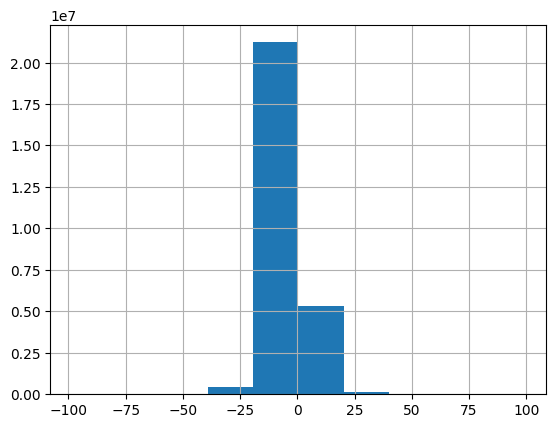
\includegraphics[width=0.49\textwidth]{images/output.png}
    \caption{Single column figure of png image, try to avoid using png, at least use PDF or better, TikZ}
    \label{fig:my_label}
\end{figure}

\blindtext \blindtext \blindtext

\begin{figure}
    \centering
    \begin{tikzpicture}
        \begin{axis}[
    		xlabel=Cost,
    		ylabel=Error
        ]
        \addplot table [x=a, y=c, col sep=comma]{data/data.csv};
        \end{axis}
    \end{tikzpicture}
    \caption{Sample figure using tikZ, we are reading from a file in data/ folder.}
    \label{fig:my_label2}
\end{figure}

\blindtext \blindtext \blindtext

\begin{figure}[t!]
    \centering
    \begin{tikzpicture}
      \begin{groupplot}[
            group style={
                group size=2 by 2,
                x descriptions at=edge bottom,
                y descriptions at=edge left,
                horizontal sep=2pt,
                vertical sep=20pt},
             ymin=0,ymax=0.75,
             scale only axis,
             title style={
                yshift=-6pt,
                fill=black!10,
                minimum width=0.4\columnwidth},
             domain=0:45, %just for example
             samples=10, %just for example
             width=0.4\columnwidth,
             height=0.3\columnwidth,
            ]
        \nextgroupplot[title=Friday]
        \addplot[scatter, only marks,mark=triangle*] {rnd};
        \nextgroupplot[title=Saturday]
        \addplot[sharp plot,mark=o] {rnd};
        \nextgroupplot[title=Sunday]
        \addplot[sharp plot,mark=square*] {rnd};
        \addplot[sharp plot,mark=square*, opacity=0.25] {rnd};
        \nextgroupplot[title=Thursday]
        \addplot[only marks,mark=o] {rnd};
        \end{groupplot}
    
        \node [left=.7cm,anchor=south,rotate=90] at ($(group c1r1.south west)!0.5!(group c1r2.north west)$) {$y$-axis label};
       \node [below=.6cm] at ($(group c1r2.south east)!0.5!(group c2r2.south west)$) {$x$-axis label};
    \end{tikzpicture}
    \caption{Sample figure using tikZ overriding default dimensions and forcing to top of the page (t!)}
    \label{fig:my_label3}
\end{figure}

\blindtext

\begin{figure*}[!t]
    \begin{subfigure}{\columnwidth}
        \centering
        \begin{tikzpicture}
        \begin{axis}[
            width=1.0\columnwidth,
            height=0.6\columnwidth,
    		xlabel=Xlabel,
    		ylabel=Ylabel
        ]
        
        \addplot [
            domain=-10:10, 
            samples=100, 
            color=red,
        ]{x^2 - 2*x - 1};
        \addlegendentry{\(x^2 - 2x - 1\)}
        \end{axis}
        \end{tikzpicture}
        \caption{Graph A}
        \label{fig:totalTemperatureAmpA}
    \end{subfigure}
    % important to not have space between
    \hfill
    % important to not have space between
    \begin{subfigure}{\columnwidth}
        \centering
        \begin{tikzpicture}
        \begin{axis}[
            width=1.0\columnwidth,
            height=0.6\columnwidth,
    		xlabel=Xlabel,
    		ylabel=Ylabel
        ]
        
        \addplot [
            domain=-10:10, 
            samples=100, 
            color=red,
        ]{-x^3 + 2*x*2 - 1};
        \addlegendentry{\(-x^3 + 2x2 - 1\)}
        \end{axis}
        \end{tikzpicture}
        \caption{graph B}
        \label{fig:totalTemperatureAmpB}
    \end{subfigure}
    \caption{Graph in subfloat environment, each figure in the subfigures will have their own caption and label.}
    \label{fig:amplitudeBC}
\end{figure*}

\begin{figure*}[!h]
    \begin{subfigure}{\columnwidth}
        \centering
        \begin{tikzpicture}
        \begin{axis}[
            width=1.0\columnwidth,
            height=0.6\columnwidth,
        ]
        
        \addplot [
            domain=-10:10,
            samples=100, 
            color=red,
        ]{x^3 - 2*x*2 - 1};
        \addlegendentry{\(x^3 - 2x2 - 1\)}
        \end{axis}
        \end{tikzpicture}
    \end{subfigure}
    % important to not have space between
    \hfill
    % important to not have space between
    \begin{subfigure}{\columnwidth}
        \centering
        \begin{tikzpicture}
        \begin{axis}[
            width=1.0\columnwidth,
            height=0.6\columnwidth,
        ]
        
        \addplot [
            domain=-10:10, 
            samples=100, 
            color=red,
        ]{-x^2 - 1*x - 5};
        \addlegendentry{\(-x^2 - x - 5\)}
        \end{axis}
        \end{tikzpicture}
    \end{subfigure}
    \caption{If you remove the caption command, then the two figures will have a single reference label (below)}
    \label{fig:amplitudeBC2}
\end{figure*}

\blindtext

\section{Algorithms}

\blindtext

\begin{algorithm}[!htbp]
    % \small
    % \scriptsize
    \begin{algorithmic}[1]
    \State $G \gets$ divide city into grids
    \State $W \gets 20$ minutes \Comment{buffer time}
    \State $F \gets \{\}$
    \ForEach {$g \in G$} \Comment{sub-areas}
        \State $I_g \gets getIncidents(I, g)$
        \State $L_g \gets getStops(L, g)$
        \ForEach{$i \in I_g$}
            \State $t_s \gets i_{time} - W$
            \State $t_e \gets i_{time} + W$
            \State $d_{pre}$ \Comment{stop-to-stop delay}
            \State $d_{post} = travelTime(t_e, e(L_j), e(L_{j+1}))$
            \State $F.append(\frac{d_{post}}{d_{pre}})$ \Comment{factor at $i_{time}$}
        \EndFor
    \EndFor
    \State \Return $F$
    \end{algorithmic}
    \caption{Stop-to-stop delays due to incidents}
    \label{algo:incident_factor}
\end{algorithm}

\section{Table}
\blindtext
% Please add the following required packages to your document preamble:
% \usepackage{graphicx}
% \usepackage[normalem]{ulem}
% \useunder{\uline}{\ul}{}
\definecolor{Gray}{gray}{0.9}
\begin{table}[!t]
\caption{Notation lookup table}
\centering
% \vspace{-0.1in}
\footnotesize

% \scriptsize
%  \fontsize{5}{6}\selectfont
% \tiny
% \captionsetup{font=smaller}
% \small
% \fontsize{5.0pt}{5.0pt}\selectfont
% \resizebox{1.0\columnwidth}{!}{%
\setlength\extrarowheight{2pt} % for a bit of visual "breathing space"
\begin{tabularx}{0.49\textwidth}{|l|X|}
\hline

{\textbf{Symbol}}     & {\textbf{Definition}}                           \\ \hline\rowcolor{Gray}
$V$                 	  & Set of vehicles                                                                               \\ \hline
$C$                       & Set of chargers                                                                               \\ \hline\rowcolor{Gray}
$\theta^t$                & Set of charging plan for all chargers, with $\theta^i_t$ denoting the plan for $c_i \in C$    \\ \hline
$\ell_t$                  & Building power consumption at time $t$                                                                              \\ \hline\rowcolor{Gray}
$S$                       & Set of states                                                                                 \\ \hline
$A$                       & Set of all feasible actions                                                                   \\ \hline\rowcolor{Gray}
$P$                  	  & State transition function                                                                     \\ \hline
$T$                       & Temporal distribution over transitions                                                        \\ \hline\rowcolor{Gray}
$R$                       & Instantaneous reward function                                                                 \\ \hline
$\gamma$                  & Discount factor for future rewards                                                            \\ \hline\rowcolor{Gray}
$vloc_t$                  & Vehicle location                                                                              \\ \hline
$c(V^i)$                  & Capacity of vehicle                                                                           \\ \hline\rowcolor{Gray}
$o(V^i_t)$                & Occupancy of vehicle at time $t$                                                              \\ \hline
$w(V^i_t)$                & Status of vehicle at time $t$                                                                 \\ \hline\rowcolor{Gray}
$C$                       & Explore and exploit parameter                                                                 \\ \hline
$E$                       & Generative model                       \\ \hline
\end{tabularx}%
% }
% \vspace{-0.2in}
\label{tab:symbols}
\end{table}


More samples for TikZ are found here: \url{https://pgfplots.sourceforge.net/gallery.html}. You can use apps like Zotero do create your references, but its often better to just get it from the actual source.